\newpage
\section{Durchführung}
\label{sec:Durchführung}
\begin{figure}
  \centering
  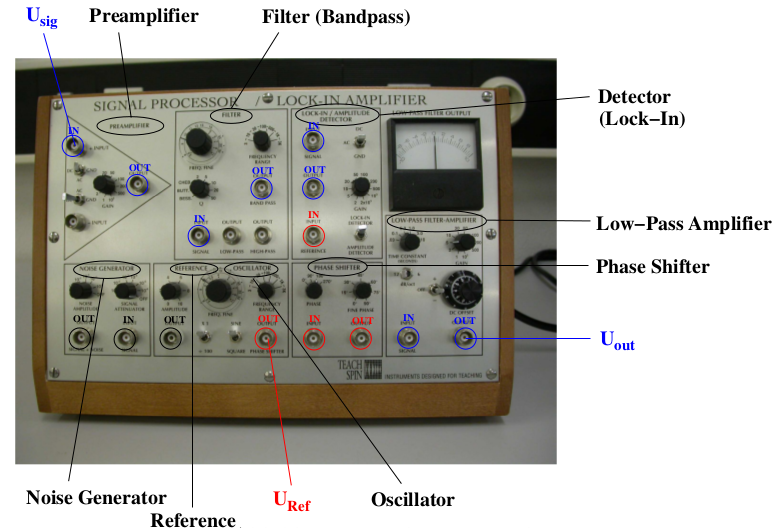
\includegraphics[width=0.8\textwidth]{verstaerker.png}
  \caption{Modularer Lock-In-Verstärker\cite{sample}.}
  \label{fig:verstaerker}
\end{figure}

{Es wird ein modularer Lock-In-Verstärker verwendet, welcher sich aus} folgenden
Elementen (auch in Abbildung \ref{fig:verstaerker} zu sehen) zusammensetzt:
Vorverstärker, Bandpassfilter, Phasenschieber, Funktionsgenerator, Rausch-Generator,
Tiefpass-Verstärker und Amplituden-/Lock-In-Detektor.

Zunächst werden die Signale des Funktionsgenerators mit Hilfe eines Speicheroszilloskops
überprüft. Dann wird nachfolgende Schaltung aufgebaut und der Rausch-Generator auf
OFF geschaltet.
\begin{figure}
  \centering
  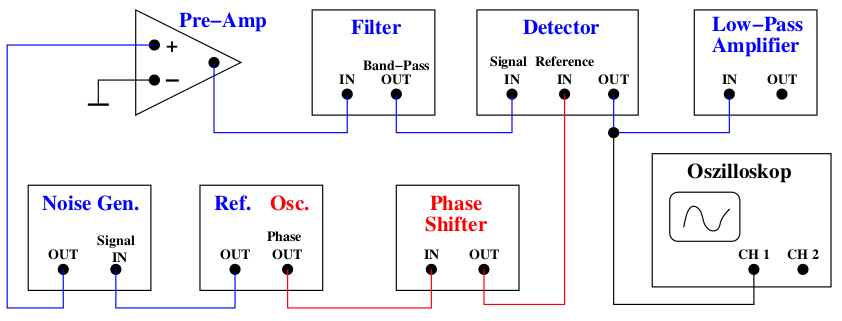
\includegraphics[width=0.8\textwidth]{schaltung.png}
  \caption{Schematischer Aufbau des Lock-In-Verstärkers\cite{sample}.}
  \label{fig:schaltung}
\end{figure}

Ein sinusförmiges Signal $U_\symup{sig}$ wird mit einem Referenzsignal
$U_\symup{ref}$ gleicher Frequenz gemischt und das Ausgangssignal für verschiedene
Phasen (je mit und ohne Integration durch den Tiefpass) graphisch dargestellt.
Desweiteren wird die Ausgangsspannung in Abhänigkeit der Phasenverschiebung
$\Delta\Phi$ gemessen.
Im nächsten Schritt werden diese Messungen wiederholt, jedoch mit eingeschaltetem
Rausch-Generator, sodass das Eingangssignal verrauscht ist.
\begin{figure}
  \centering
  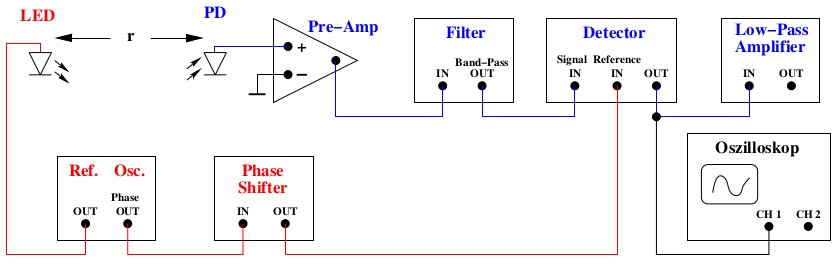
\includegraphics[width=0.8\textwidth]{photodetektor.png}
  \caption{Schematischer Aufbau der Photodetektorschaltung\cite{sample}.}
  \label{fig:photodetektor}
\end{figure}
Zuletzt wird eine Photodetektorschaltung nach Abbildung \ref{fig:photodetektor}
aufgebaut und die Lichtintensität der Leuchtdiode (LED) in Abhänigkeit des Abstandes
r zwischen der LED und der Photodiode gemessen, sowie der maximale Abstand bestimmt,
bei dem das Licht noch nachgewiesen werden kann.
